\documentclass[pdftex,bezier,german,a4,twoside, headexclude,12pt,nochapterprefix, titlepage]{extarticle}
\usepackage[utf8]{inputenc}
\usepackage[paper=a4paper,margin=2.5cm]{geometry}
\usepackage[english]{babel}
\usepackage{multicol}
\usepackage{relsize}
\include{mathphys}
\usepackage{graphicx}
  \graphicspath{{./fig/}}
\usepackage{amsmath}
\usepackage{amssymb}
\usepackage[table]{xcolor}
\usepackage{booktabs}
\usepackage{color}
\usepackage{textcomp}
\usepackage{cite}
\usepackage{caption} 
\usepackage{braket}
\usepackage{float}
\usepackage{subfigure}
\usepackage[hidelinks=true]{hyperref}
\usepackage{placeins}
%===========================================================================
\def\captionsize{\small}

\usepackage{setspace}
\doublespace

\restylefloat{figure}
\pagestyle{plain}

\setlength{\parindent}{0ex}
\setlength{\parskip}{1ex}

%% Listings
\usepackage{color}
\usepackage{listings}
\usepackage{courier}
\definecolor{darkgreen}{rgb}{0 0.4 0}
\lstset{
         basicstyle=\footnotesize\linespread{1}\ttfamily,% Standardschrift
         numbers=left,               % Ort der Zeilennummern
         numberstyle=\tiny,          % Stil der Zeilennummern
         stepnumber=1,               % Abstand zwischen den Zeilennummern
         numbersep=1pt,              % Abstand der Nummern zum Text
         tabsize=2,                  % Groesse von Tabs
         extendedchars=true,         %
         %breaklines=true,            % Zeilen werden Umgebrochen
         keywordstyle=\color{blue},
 %        keywordstyle=[1]\textbf,    % Stil der Keywords
 %        keywordstyle=[2]\textbf,    %
 %        keywordstyle=[3]\textbf,    %
 %        keywordstyle=[4]\textbf,   \sqrt{\sqrt{}} %
         %stringstyle=\color{magenta}\ttfamily, % Farbe der String
         %showspaces=false,           % Leerzeichen anzeigen ?
         %showtabs=false,             % Tabs anzeigen ?
         numbers=none,
         numbersep=2pt, 
         showstringspaces=false      % Leerzeichen in Strings anzeigen ?        
 }
 \lstloadlanguages{% Check Dokumentation for further languages ...
         C,
         Matlab
 }
 \lstdefinestyle{Matlab}{
         commentstyle=\color{darkgreen}\ttfamily, % Farbe der String
 }
%\DeclareCaptionFont{blue}{\color{blue}} 

%\captionsetup[lstlisting]{singlelinecheck=false, labelfont={blue}, textfont={blue}}

\renewcommand\lstlistingname{Script}
\def\algorithmautorefname{Algorithm}


% ================== ALGORITHM ==================
\newcounter{algorithm}
%\renewcommand{\thealgorithm}{\thesection.\arabic{algorithm}}% Algorithm counter definition
\newcommand{\algorithmprehook}[2]{%
  \refstepcounter{algorithm}% Increment counter for correct reference
  \listingcaption{Algorithm}{#1}% Algorithm caption
  \label{#2}% Label algorithm
}
\lstnewenvironment{algorithm}[3][]{% \begin{algorithm}[<listings options>]{<caption>}{<label>}...
  \algorithmprehook{#2}{#3}% Algorithm pre-hook
  \lstset{#1}% Set listings options
} {}% ...\end{algorithm}
\def\algorithmautorefname{Algorithm}% Autoref caption

\newcommand{\simpel}{\textsf{SimPel}}
\newcommand{\glopel}{\textsf{GloPel}}
\newcommand{\figspace}{\hspace{0.5cm}}

\begin{document}

\begin{titlepage}
\centering

\vspace*{3em}

\rule{\textwidth}{2pt}
\\[1.5em]
\textbf{\Large \simpel{} User Manual}
\\[1em]
{\large Version 1.0.0}
\\[1em]
\rule{\textwidth}{2pt}

\vspace*{3em}


\includegraphics[scale=0.65]{SimPel_Logo.pdf}

\vspace*{3em}

by \\[1em]
{\Large Stephan Rein}\\[2em]
{\large \url{https://www.glopel.de/}}

\end{titlepage}


\tableofcontents

\clearpage

\section*{Preface}

\simpel{} has been developed in the group of Prof. Dr. Stefan Weber at the University of Freiburg, Freiburg im Breisgau, Germany, during the last couple of years in course of developing \glopel, a software for advanced global analysis of PELDOR/DEER spectra.

This manual describes the general usage of \simpel{} and gives an overview of the maths behind that has been implemented.

If you use \simpel{} for your own research and publish results accordingly, please give credits citing the appropriate reference:

\begin{quote}\small
Stephan Rein, Philipp Lewe, Susana L. Andrade, Sylwia Kacprzak, Stefan Weber
\\
Global analysis of complex PELDOR time traces
\\
\emph{Journal of Magnetic Resonance}, submitted 
\end{quote}


%\subsection*{Acknowledgments}

A number of people have helped shaping \simpel{} and the ideas behind. First and foremost, Dr. Sylwia Kacprzak (now Bruker Biospin) was for years the driving force behind \simpel{} due to the need for advanced analysis of PELDOR/DEER data with limited signal-to-noise ratio. Dr. Till Biskup contributed ideas for programming and details of the implementation that make all the difference between a program useful for a larger audience and a simple in-house solution. And finally, without Prof. Dr. Stefan Weber and his continuous and continuing support, this work would not have been possible.

\vspace*{2em}

\begin{flushright}
Freiburg, March 2018\\
Stephan Rein
\end{flushright}

\clearpage


\section{Introduction}

\subsection{General Description}

\simpel{} is a Python3-based simulation program for high-performance simulations of PELDOR/DEER traces. \simpel{} provides a user-friendly GUI based on the PyQt5 GUI framework.

Up to five Gaussian distributions with independent linear coefficients and standard deviations can be used for creating a distance distribution. The user-defined distance distribution is used to calculate the PELDOR/DEER trace. Many simulation options are available. In addition to the pure dipolar evolution signal of the PELDOR/DEER trace, a background function can be added as well as Gaussian (white) noise. Simulations can be saved and automatic figure export is supported (formats: png, tif, pdf, ....).

Configuration settings for simulation and plotting options can be adjusted, allowing the user, e.g. to create figures with own preferences.

\simpel{} can be used to systematically explore the impact of changes of the distance distribution on the PELDOR/DEER trace. Additionally \simpel{} can be used to compare experimental time traces with simulations.

The Bruker BES3T file format (.DTA, .DSC) used by Xepr and Elexsys spectrometers
is supported as well as text files for loading experimental data. Furthermore, \simpel{} can be used to create high quality figures for simulated time traces and distance distributions.

For PELDOR/DEER analysis, we recommend the program GloPel, which is also freely available and can be downloaded from {\url{https://www.glopel.de/}}.

\subsection{License}

\simpel{} is made available free of charge and open source. 
\simpel{} is distributed under a 2-clause license (“Simplified BSD License” or “FreeBSD License”). The full text of this license can be found in the file \texttt{LICENSE.txt} in the main directory of the SimPel source code.


\subsection{Requirements}

TBD


\subsection{Installation Instructions}

\simpel{} is available free of charge and open source (see license). We recommend everybody with a recent Python installation on their computers to download the source code and use it. 
However, 
\simpel{} can be downloaded as executable binary for Windows, macOS and several Linux flavors.
It was tested on various systems including Windows 7 (32-bit and 64-bit architecture), Windows 10 (32-bit and 64-bit architecture), macOS 10.12.6 (Sierra),
and Ubuntu 16.04.\\

Please note that these versions are much harder to debug if something goes wrong, therefore, they are provided as is without any further support. 



A note on how these binaries have been created: Thanks to PyInstaller, it is rather straightforward to create binary distributions
of Python programs, both as directories with all the necessary files contained as well as single-file executables. 
Similar to cx\_freeze, PyInstaller allows to define additional options in a “spec” file. 
This file is included in the sources available. To get a one-file binary, it was called simply as follows:\\
\begin{lstlisting}[language=bash]
  pyinstaller --onefile --noconsole setup.spec
\end{lstlisting}
\begin{enumerate}
\item Binaries for Linux have been built with Ubuntu 16.04 (Xenial Xerus) and a Python installation consisting of Python 3.5, matplotlib 2.1.1, PyQt 5.8.2,  NumPy 1.13.3, SciPy 0.17.0
\item  Binaries for macOS have been built with macOS 10.12.6 (Sierra) and a Python installation consisting of Python 3.5, matplotlib 2.0.0, PyQt 5.8.2
 \item  Binaries for Windows have been built with Windows7 (32-bit architecture) and a Python installation consisting of Python 3.5, matplotlib 2.1.2, NumPy (+MKL) 1.11.3, SciPy 0.19.0, PyQt 5.8.2
\end{enumerate}


\newpage
\section{Using \simpel}
\FloatBarrier
\subsection{Basic Options}
When starting \simpel, the main GUI (\autoref{MainWindowfig}) opens. Default settings for all parameters are loaded when starting
the program. The main GUI window as well as all additional windows are resizable and can be adjusted by the user.
\begin{figure}[h!]
\begin{center}
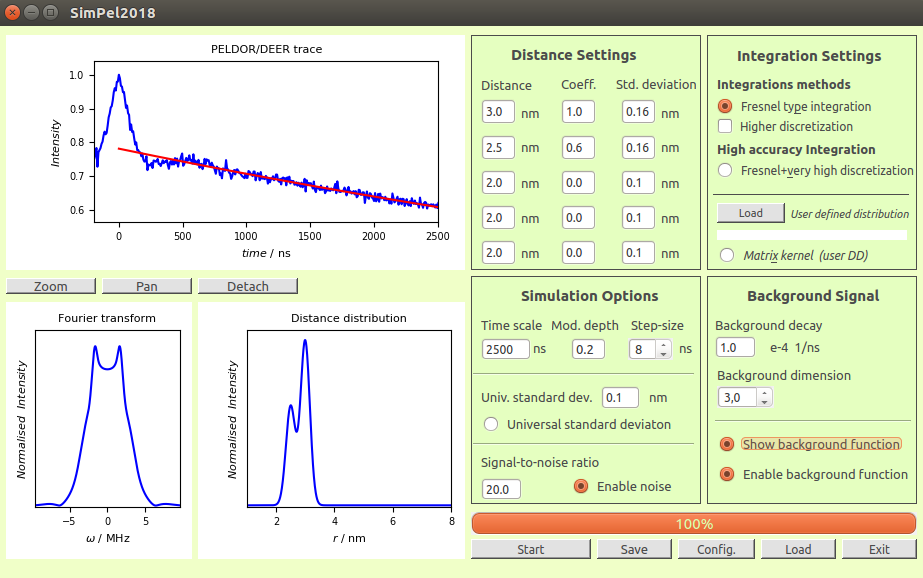
\includegraphics[scale=0.5]{Main_Window_example.png}
\caption{Main GUI window of \simpel{} running on a Linux system (Ubuntu 16.04). Simulation of a bimodal distance distribution is shown. A background
function (shown in red) was enabled. White noise was added to the simulated time trace.}
\label{MainWindowfig}
\end{center}
\end{figure}
Parameters such as central distances $r_{0,i}$, standard deviations $\sigma_i$, or linear coefficients $c_i$ for up to five
Gaussian functions can be set by the user. Additional simulation options are the time scale ($t_{\mathrm{max}}$), the 
PELDOR/DEER step-size and the modulation depth $\lambda$. The PELDOR trace is calculated according to  \autoref{PELDOR_kernel_function}.
A background function can be added to the PELDOR/DEER trace. The background dimension 
can be chosen between 1 and 6 in steps of 0.1. The background decay constant can be defined by the user. The background function is calculated according to \autoref{background_function}. White noise can be added by enabling the corresponding button. The signal-to-noise
ration can be given by the user.
The simulation is carried out by pressing the ``Start'' button. 

A user-defined distance can be loaded. From this distance distribution the PELDOR/DEER trace is calculated using a kernel matrix according to
\autoref{kernel_matrix_cal}. The distance distribution has to be provided as text file.

Experimental PELDOR/DEER time traces can be loaded and compared to simulations. \simpel{} accepts either a text-file format
or a Bruker BES3T file format (.DTA, .DSC). Example for a comparison between an experimental dataset and a simulation is shown in
\autoref{Expample_experimental_dataset}

\begin{figure}[!htb]
\centering
     \subfigure{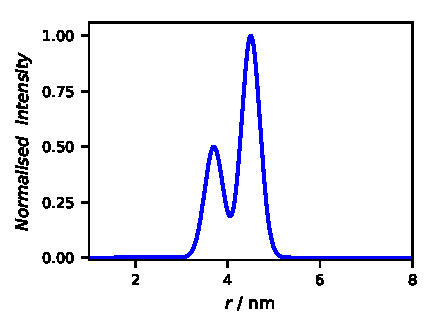
\includegraphics{Test_5_Distance_distribution.pdf}}\figspace
     \subfigure{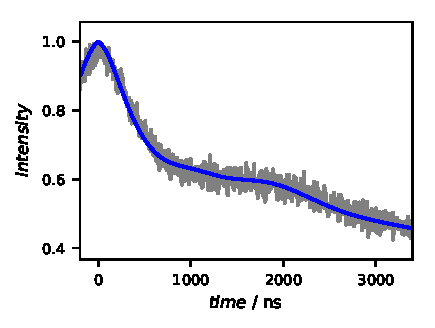
\includegraphics{Test_5_Time_trace.pdf}} \\[-0.3cm]
    \caption{Comparison of a simulation (blue) and an experimental time trace (gray). \simpel{} can be used to get a first impression about the distance distribution of an experimental time trace. For detailed analysis, we recommend to use the program GloPel (\url{www.glopel.de}).
    }
\label{Expample_experimental_dataset}
\end{figure} 
\FloatBarrier
\newpage
\subsection{Integration Settings}
The standard  integration method of \simpel{} uses:
\begin{align*}
k =  19+(\mathrm{round}(100\sigma_i)) + (20+(\mathrm{round}(100\sigma_i))\%2
\end{align*}
points for the discretization of a Gaussian function $f_i$ in the interval
$[r_{0,i}-3\sigma_i \ ,\ r_{0,i}+3\sigma_i]$. This is sufficient for most time traces. However, for some cases, especially
if broad distance distributions are present in the small distance region, this is not sufficient and simulation noise is observed
(\autoref{Integration_mehtods_comparison}).
\begin{figure}[!htb]
\centering
     \subfigure{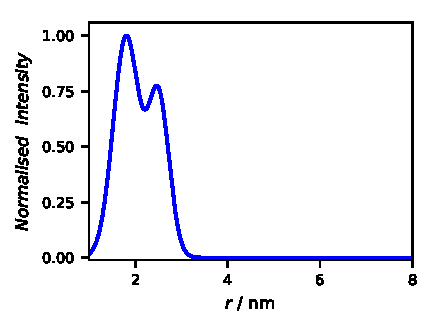
\includegraphics{Test_1_Distance_distribution.pdf}}\figspace
     \subfigure{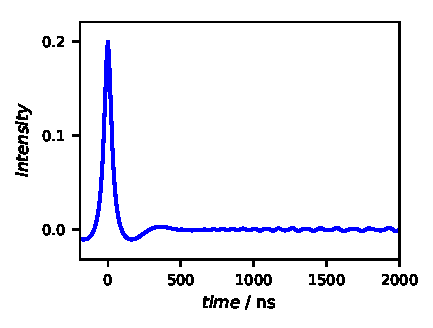
\includegraphics{Test_1_Time_trace.pdf}} \\[-0.3cm]
     \subfigure{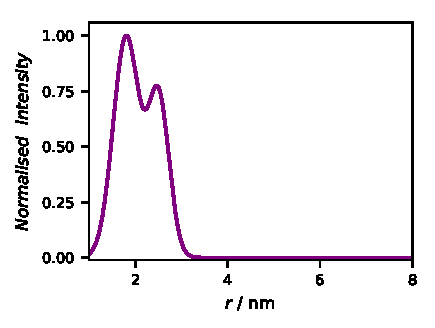
\includegraphics{Test_2_Distance_distribution.pdf}}\figspace
     \subfigure{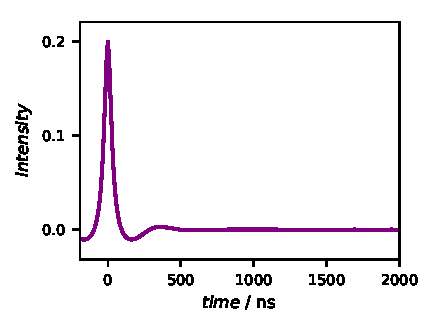
\includegraphics{Test_2_Time_trace.pdf}}
    \caption{Comparison of standard integration settings (top, blue) and integration with higher discretization of the Gaussian
    functions (bottom, purple) used for simulation.
    }
\label{Integration_mehtods_comparison}
\end{figure} 
This simulation noise  can be avoided by enabling the ``Higher discretization'' check-box (three times higher discretization rate) or by checking/enabling
``Fresnel+very high discretization'' button (five times higher discretization rate). These should be sufficient for acquiring noise-free
simulations of all possible distance distributions.

\newpage
\subsection{Data Output and Figure Export}
Once a simulation was carried out, the result can be saved and the figures exported. If the ``Save'' button is clicked, a
file manager opens and the files can be saved at the  location defined by the user (\autoref{Save_output_example}).
The PELDOR/DEER trace, the distance distribution, and the Fourier transform are saved as text files. Additionally,
an information sheet is automatically created, containing all simulation options (\autoref{Information_sheet}).
The information sheet contains all information to reproduce the simulation. Naturally, white noise cannot
be reproduced exactly as it is created via a pseudo-random number generator.
\begin{figure}[!htb]
\centering
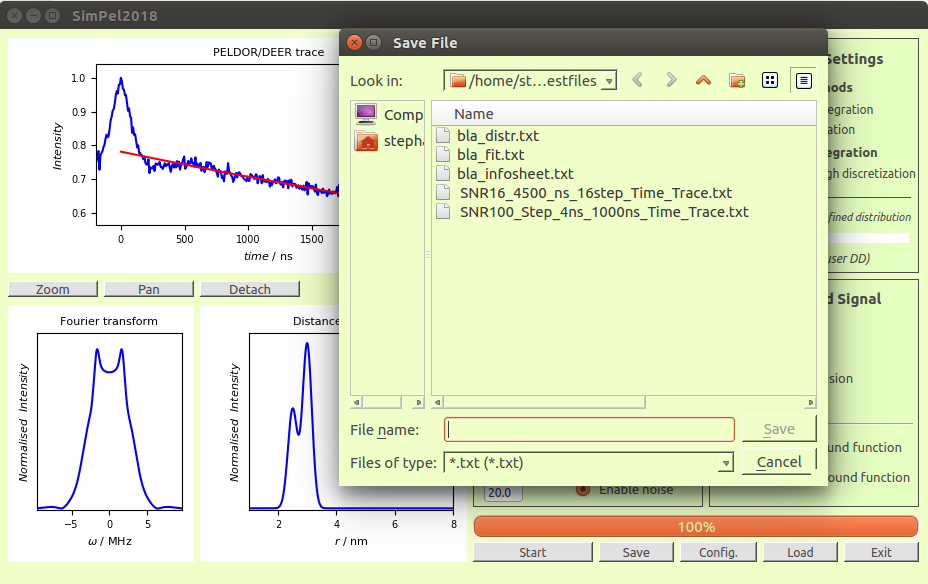
\includegraphics[scale=0.5]{Save_output_example.png}
    \caption{File manager opens when the Save button is clicked. All output files are saved as text-files.
    }
\label{Save_output_example}
\end{figure} 
If not disabled in the configurations (for configuration settings see next section) the figures are automatically
saved as Portable Network Graphics (png) and  as vectorized Portable Document Format (PDF) files.

\newpage
\begin{lstlisting}[caption={Example for an automatically aved information sheet.},label = Information_sheet]

Infosheet for PELDOR/DEER Simulation. Original Path:
/home/stephan/Python_SimPel/Test_output_1

Simulated with SimPel2018: 1.0.0

Analyzed at: 2018-03-16 11:00:44

*************Simulation Parameter*****************

Distance / nm 	 Coefficient	  sigma / nm
1.8000	         1.0000	          0.2800	         
2.5000	         0.6000	          0.2300	         
2.0000	         0.0000	          0.1000	         
2.0000	         0.0000	          0.1000	         
2.0000	         0.0000	          0.1000	         


PELDOR/DEER step size: 8.0 ns

PELDOR/DEER time scale: 2000.0 ns

PELDOR/DEER modulation depth: 0.2

Gaussian noise enabled: False

Background function enabled: False

Integration method: Fresnel integrals
\end{lstlisting}



\newpage
\FloatBarrier
\subsection{Configuration Settings}
Many standard settings of \simpel{} can be changed either dynamically directly in the GUI or as default by creating a
configuration file.\\
The current configuration can be opened and changed when running  \simpel{} by pressing the ``Config.'' button.
If new configurations are set and the ``Accept'' button (see \autoref{Config_settings})
is clicked, the new settings are adapted immediately and a new simulation is carried out.
\begin{figure}[!htb]
\centering
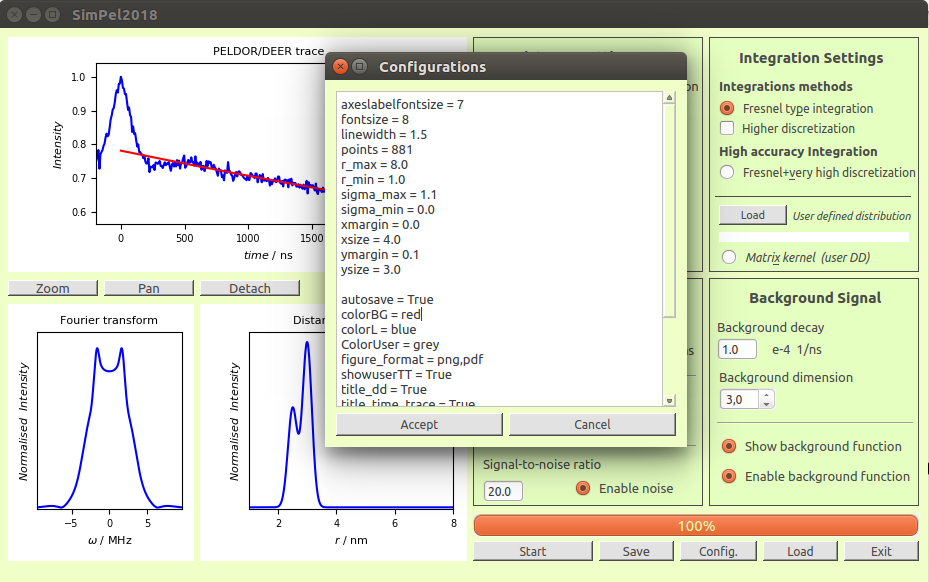
\includegraphics[scale=0.5]{Config_example.png}
    \caption{Current configurations of  \simpel. They can be easily altered and accepted.}
   \label{Config_settings}
\end{figure}
Alternatively, user defined configuration setting can be saved in a file called \texttt{SimPel.conf}. This configuration file
needs to be located in the folder containing the executable or the source code. An example of a user defined \texttt{SimPel.conf} is
shown in \autoref{user_config_list} and the corresponding changes on the figures are demonstrated in \autoref{Different_config_figures}.
\newpage
\begin{lstlisting}[caption={Example for a user defined configuration file (\texttt{SimPel.conf}).},label = user_config_list]

#User defined default configurations 
r_max = 10
r_min = 2
t_min = 0
fontsize = 9.0
Lcolor = green
title_dd = False
title_time_trace = False
yticks_dd = True
ylabel_time_trace = $Form\ \ factor$
\end{lstlisting}

\begin{figure}[!htb]
\centering
     \subfigure{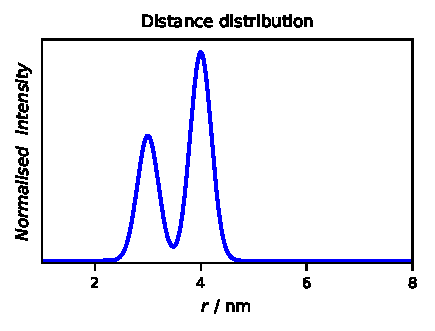
\includegraphics{Test_3_Distance_distribution.pdf}}\figspace
     \subfigure{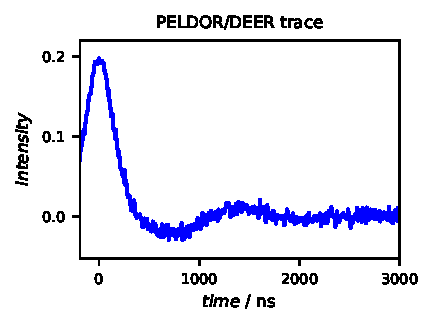
\includegraphics{Test_3_Time_trace.pdf}} \\[-0.3cm]
     \subfigure{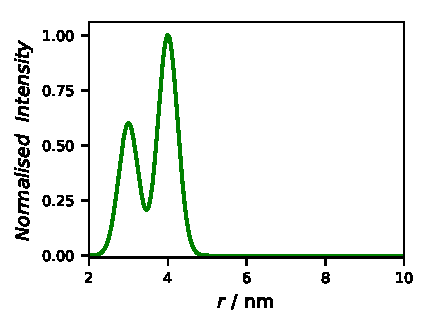
\includegraphics{Test_4_Distance_distribution.pdf}}\figspace
     \subfigure{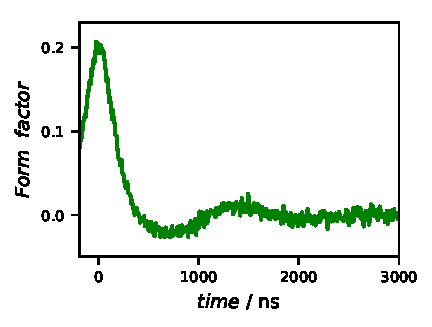
\includegraphics{Test_4_Time_trace.pdf}}
    \caption{Comparison of standard configurations of \simpel{} (top, blue) and user-defined default configurations as set in \autoref{user_config_list}. Many settings were changed compared to the standard configuration (the fontsize was increased, the distance range and color were changed, ....).}
\label{Different_config_figures}
\end{figure} 



\subsection{Detaching Figures}
If wished, the plots can be detached. This enables additional options to modify or configure the plots.
If new simulations are carried out
or other things are changed, e.g. noise is added, the figures are updated automatically.
\begin{figure}[h!]
\begin{center}
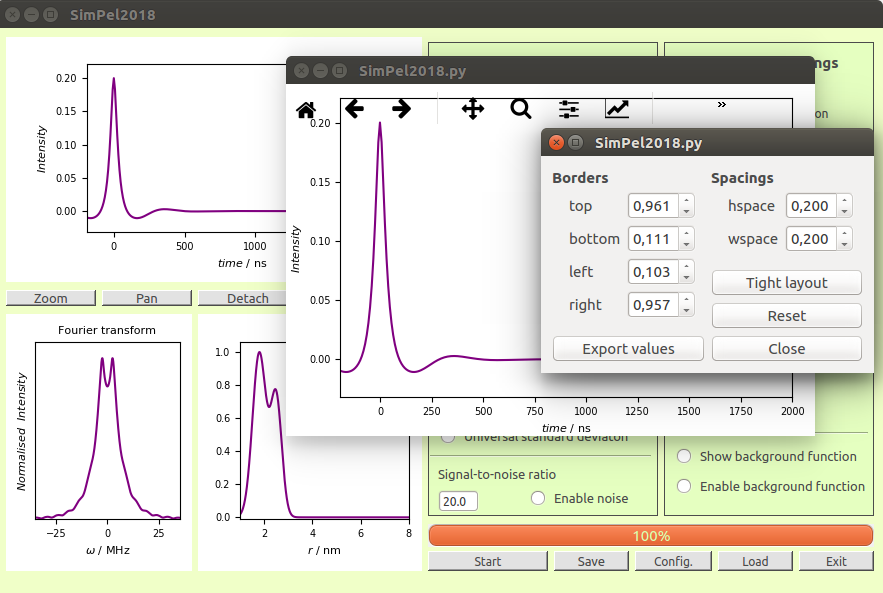
\includegraphics[scale=0.5]{Detach_figures.png}
\caption{Main GUI window of \simpel{} running on a Linux system (Ubuntu 16.04). Detached figures can be modified separately and saved afterwards.}
\label{Detach_figure}
\end{center}
\end{figure}

\clearpage

\section{Algorithms for the Calculation of PELDOR/DEER Traces}


\subsection{PELDOR/DEER Trace Simulation Kernel}

\simpel{} calculates a PELDOR/DEER time trace $V(t)$ using:
%
\begin{align}
\begin{split}
& \boldsymbol{V}=  \lambda \sum_{i=1}^5 c_i\sum_{k=1}^{j}I(r_{i,k})S(\omega_{i,k},t) \\
&\mbox{with}\hspace{0.5cm} j =  19+(\mathrm{round}(100\sigma_i)) + (20+(\mathrm{round}(100\sigma_i))\%2,\\
&\mbox{with}\hspace{0.5cm} I(r_{i,k}) =\dfrac{1}{N_{i}} \;
\mathrm{exp}\left[-\frac{1}{2}\left(\frac{r_{i,0}-r_{i,k}}{\sigma_i}\right)^2\right],\\
&\mbox{with}\hspace{0.5cm} N_{i} = \sum_{k=1}^{j}\mathrm{exp}\left[-\frac{1}{2}\left(\frac{r_{i,0}-r_{i,k}}{\sigma_i}\right)^2\right] ,\\
&\mbox{with}\hspace{0.5cm}S(\omega_{i,k}) = 
\frac{\cos{\big(\omega_{i,k}|t| \big)}}{z_{i,k}} \cdot \text{FresnelC}(z_{i,k})  + 
   \frac{\sin{\big(\omega_{i,k} |t|\big)}}{z_{i,k}} \cdot \text{FresnelS}(z_{i,k}),\\
  &\mbox{with}\hspace{0.5cm}  z_{i,k} = \sqrt{\frac{6\,\omega_{i,k} |t| }{\pi}},\\
&\mbox{with}\hspace{0.5cm} \omega_{i,k} = \dfrac{52.04\cdot 2 \pi}{r_{i,k}^3},\\ 
&\mbox{with}\hspace{0.3cm} \sum_{k=1}^{5}c_i = 1 \hspace{0.3cm}
\mbox{and}\hspace{0.3cm}c_i \in\mathbb{R}^+_0\; .
\label{PELDOR_kernel_function}
\end{split}
\end{align}

$\lambda$ is the given modulation depth, $r_{i,0}$ are the five given central distances, $\sigma_i$ are the given standard deviation, $c_i$ are the linear coefficients and $t$ is the time vector running from -200~ns to the user-defined value of $t_{\mathrm{max}}$ with a user-defined step size. The linear coefficients are renormalized to their sum being equal to one. It is therefore not necessary to pay attention to the normalization of the linear coefficients.
The normalization factor for a Gaussian function $\left(\dfrac{1}{\sigma_i \sqrt{2\pi}}\right)$ is not used. Instead the Gaussian functions are normalized to their sum. This is more exact, as different standard deviations cause different discretization rates for different standard deviations. The PELDOR kernel integral is not evaluated directly to avoid numerical integration. Instead, the integral is reformulated as a sum of Fresnel integrals (FresnelC and FresnelS, see \autoref{Fresnel_int}). The Fresnel integrals can be evaluated in vectorized form by passing a multidimensional array to the SciPy function
\texttt{fresnel} (scipy.special.fresnel). Indeed, the full PELDOR/DEER trace calculation shown in \autoref{PELDOR_kernel_function} is carried out without a loop but by passing a 3-dimensional array ($i,k,t$) to the Fresnel function.
%
\begin{eqnarray}
\begin{split}
S(\omega_{\text{D}},t) & = \int\limits_{0}^{\pi/2}\mathrm{cos}\Big((1-3\,\mathrm{cos}^2\phi)\,\omega_{\text{D}}\,t\Big)\sin \phi\; \text{d}\phi \\ 
   & = 
   \frac{\cos{\big(\omega_{\text{D}}t \big)}}{z} 
   \underbrace{\int\limits_{0}^{z} \cos{\left( \frac{\pi}{2}\,u^{2} \right)} 
   \;\text{d}u}_{\equiv \text{FresnelC}(z)} \; + \; 
   \frac{\sin{\big(\omega_{\text{D}} t \big)}}{z}
   \underbrace{\int\limits_{0}^{z} 
   \sin{\left( \frac{\pi}{2}\,u^{2} \right)}\;\text{d}u}_{\equiv \text{FresnelS}(z)}      
\label{eqFresnel08} \\[2mm]
   & =  \frac{\cos{\big(\omega_{\text{D}}t \big)}}{z} \cdot \text{FresnelC}(z) \; + \;
   \frac{\sin{\big(\omega_{\text{D}} t\big)}}{z} \cdot \text{FresnelS}(z)\; ,
   \quad\text{with}\;\; z = \sqrt{\frac{6\,\omega_{\text{D}} t }{\pi}}
\label{eqFresnel09}  
\end{split}
\label{Fresnel_int}
\end{eqnarray}


\vspace*{1em}

\subsection{PELDOR/DEER Trace Kernel Matrix}

If a user-defined distance distribution $\boldsymbol{P} = r_{i}$ is loaded and the PELDOR/DEER trace has to be calculated, a matrix kernel $\boldsymbol{K}$ is used:
%
\begin{align}
\begin{split}
&V(t) = \boldsymbol{K}\boldsymbol{P},\\
&\mbox{with}\hspace{0.5cm} \boldsymbol{K} = K_{ji} =
\frac{\cos{\big(\omega_{i}|t_j| \big)}}{z_{i}} \cdot \text{FresnelC}(z_{i})  + 
   \frac{\sin{\big(\omega_{i} |t_j|\big)}}{z_{i}} \cdot \text{FresnelS}(z_{i}),\\
  &\mbox{with}\hspace{0.5cm}  z_{i} = \sqrt{\frac{6\,\omega_{i} |t_j| }{\pi}},\\
&\mbox{with}\hspace{0.5cm} \omega_{i} = \dfrac{52.04\cdot 2 \pi}{r_{i}^3},\\ 
\label{kernel_matrix_cal}
\end{split}
\end{align}

The calculation of the kernel matrix $\boldsymbol{K}$ is carried our by passing a 2-dimensional array to the Fresnel function of SciPy. This allows a highly efficient calculation of the kernel matrix.


\subsection{Adding a Background Function}

A background function can be ``added'' to the PELDOR kernel function, resulting in the new function $V_{b}(t)$: 

\begin{align}
\begin{split}
&V_{b}(t) = (V(t)+1-\lambda)B(t), \\
&\mbox{with}\hspace{0.5cm}B(t) = \mathrm{exp}\left[-k|t^{d/3}|\lambda \right]
\label{background_function}
\end{split}
\end{align}

$k$ is the user-defined background decay constant and $d$ is the user-defined background dimension. The 
function $V_{b}(t)$ is subsequently normalized to its maximum.
The simulation function without background decay is kept as variable. It is therefore not necessary to rerun a simulation in 
case the background settings are changed.


\subsection{Adding White Noise}

The noise used is statistical (uncorrelated) noise, having a probability density function (PDF) equal to that of a normalized Gaussian function.
It can be described as additive white Gaussian noise (AWGN). The noise is added to get a noisy time trace $V_n(t)$:
\begin{align}
\begin{split}
 & V_n(t) = V(t)+n,\\
 &\mbox{with}\hspace{0.5cm} n = \dfrac{\lambda}{\text{SNR}} \; p_n(x), \\
 &\mbox{with}\hspace{0.5cm} p_n(x) = \left(\dfrac{1}{\sigma_n \sqrt{2\pi}}\right)
 \mathrm{exp}\left[-\frac{1}{2}\left(\frac{x}{\sigma_n}\right)^2\right]
 \end{split}
\end{align}
This implies a mean value of $0$. SNR is the given signal-to-noise ratio and $\sigma_n$ is set to one.
The noise-free simulation is kept as variable. Therefore, it is not necessary to rerun a simulation when removing the noise again or
changing the signal-to-noise level.


\newpage

\section{Full configuration file (\texttt{SimPel.conf})}

\begin{lstlisting}[caption={Complete configuration file of the default settings of SimPel},label = full_config_list]

# Simulation Settings
r_max = 8
r_min = 1
sigma_max = 1.1
sigma_min = 0.0
points = 881
t_min = -200

# Figure Settings
fontsize = 9
axeslabelfontsize = 8
xmargin = 0.0
ymargin = 0.1
xsize = 4
ysize = 3 
colorL = blue
colorBG = red
ColorUser = grey
linewidth = 1.5
showuserTT = True
yticks_time_trace = True
yticks_dd = False
title_time_trace = True
title_dd = True

# Individual Axes Labels (Latex Math Environment Syntax)
ylabel_time_trace = $Intensity$
xlabel_time_trace = $time\ \mathrm{/ \ ns}$
ylabel_dd = $Normalised\ \ Intensity$
xlabel_dd =$r\ \mathrm{/ \ nm}$

#Save figures
autosave = True
figure_format =png,pdf
\end{lstlisting}
\end{document}
